\section{Semaphore}

\begin{frame}{Semaphore}
\begin{columns}
\begin{column}{0.5\textwidth}
\includegraphics[height=0.5\textheight,angle=-90]{BhfEpfenhofen_Ausfahrsignale_Talaufwaerts_II.JPG}

{\tiny \copyright 
\url{upload.wikimedia.org/wikipedia/commons/0/0b/BhfEpfenhofen\_Ausfahrsignale\_Talaufwaerts\_II.JPG}}
\end{column}
\begin{column}{0.5\textwidth}
 \begin{itemize}
  \item \cod{down}: Signal zu
  \begin{itemize}
   \item warten
  \end{itemize}
  \item \cod{up}: Signal offen
  \begin{itemize}
   \item fahren
  \end{itemize}
 \end{itemize}
\end{column}
\end{columns}
\end{frame}

\begin{frame}{Tasklet-Semaphore}
\includegraphics[width=10cm]{tasklet-semaphore.pdf}
\end{frame}

\subsection{gpio-4.c}

\begin{frame}{gpio-4.c}{schrittweise}
 \begin{itemize}
  \item Definition global 
     \href{https://elixir.bootlin.com/linux/latest/source/include/linux/semaphore.h\#L16}
          {\cod{semaphore}}
  \item Initialisation
  
   \href{https://elixir.bootlin.com/linux/latest/source/include/linux/semaphore.h\#L32}
        {\cod{sema\_init}} anfangs geschlossen 
  \item Im Tasklet
   \href{https://elixir.bootlin.com/linux/latest/source/include/linux/semaphore.h\#L44}
        {\cod{up}}: �ffne
  \item Im \cod{get\_swi}
   \href{https://elixir.bootlin.com/linux/latest/source/include/linux/semaphore.h\#L39}
        {\cod{down}}: warte \& schliesse
 \end{itemize}
\end{frame}

\section{Wait-Queue}

\begin{frame}{Wait queue}{Task/processe warten}
\includegraphics{queue.pdf}

\vspace{5mm}
\includegraphics[width=0.25\textwidth]{queue-legend.pdf}
\end{frame}

\subsection{gpio-5.c}
\begin{frame}{gpio-5.c}{schrittweise}
 \begin{itemize}
  \item Definition global
  \begin{itemize}
   \item \href{https://elixir.bootlin.com/linux/latest/source/include/linux/wait.h\#L34}
              {\cod{wait\_queue\_head}}
   \item \cod{swiN} die Anzahl Schaltungen von \cod{swi}
  \end{itemize}
  \item go to wait
  \begin{itemize}
   \item  \href{https://elixir.bootlin.com/linux/latest/source/include/linux/wait.h\#L442}
               {\cod{wait\_event\_interruptible}}
  \end{itemize}
  \item wakeup
  \begin{itemize}
    \item \href{https://elixir.bootlin.com/linux/latest/source/include/linux/wait.h\#L201}
               {\cod{wake\_up\_interruptible}}
  \end{itemize}
 \end{itemize}
\end{frame}

\section{Semaphore-Queue}

\begin{frame}{Mit eigener {\em Semaphhore-queue}}
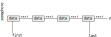
\includegraphics{semaphore-queue.pdf}
\vspace{-5mm}
\begin{itemize}
 \item put
  \begin{itemize}
   \item f�ge hinten an \cod{put}: data: Zustand des Schalters: \cod{on$|$off}
   \item �ffne Semaphore
  \end{itemize}
 \item get
 \begin{itemize}
  \item warte am Semaphore
  \item hole \cod{get} 
 \end{itemize}
\end{itemize}
\end{frame}


\subsection{Simply Linked List}
\begin{frame}{Die {\em Queue}}{einfach verlinkte Liste}
\includegraphics{queue-generic.pdf}
\end{frame}


\begin{frame}{Die {\em Queue}}{put}
\begin{block}{before}
\includegraphics{put-before.pdf}
\end{block}
\begin{block}{after}
\includegraphics{put-after.pdf}
\end{block}
\end{frame}

\begin{frame}{Die {\em Queue}}{get}
\begin{block}{before}
\includegraphics{get-before.pdf}
\end{block}
\begin{block}{after}
\includegraphics{get-after.pdf}
\end{block}
\end{frame}

\subsection{queue.c}

\begin{frame}{Verlinkte Listen}{Kommen immer wieder vor}
\begin{itemize}
 \item im userspace
 \item \cod{struct}
 \item \cod{init\_} 
 \item \cod{put\_}
 \item \cod{get\_}
  \item Dynamisches Memory
  \begin{itemize}
   \item  \cod{malloc}
   \item \cod{free}
  \end{itemize}
\end{itemize}
\end{frame}

\subsection{gpio-6.c}

\begin{frame}{Die Semaphore-Queue}
 \begin{itemize}
  \item \cod{struct} f�r Semaphore-Queue
  \item \cod{init\_} 
  \item \cod{put\_}
  \item \cod{get\_}
  \item Dynamisches Memory
  \begin{itemize}
   \item  \cod{kmalloc}
   \item \cod{kfree}
  \end{itemize}
 \end{itemize}
\end{frame}

\begin{frame}[fragile]{TODO's}{Im Zusammenhang mit den Interrups}
 \begin{itemize}
  \item mehr Informationen in \cod{buf} von \cod{get\_swi} zur�ckgeben: 
  \begin{lstlisting}
  struct SWIInfo
  {
   time_t   when;
   unsigned nbr;  //the number of switching
   unsigned state; //on|off
  };
  \end{lstlisting}
 \item Queue als {\em ringbuffer}
 \end{itemize}
\end{frame}

\subsection{TODO Mehr Info:gpio-8.c}

\begin{frame}{\cpp gemacht mit \c}
 \begin{itemize}
  \item \cod{src/queue-a-la-cpp.c}
 \end{itemize}
\end{frame}

\begin{frame}[fragile]{SWIInfo}
\begin{lstlisting}
typedef struct SWIInfo
{
 time_t       when;
 unsigned     nbr;
 unsigned     state;
} SWIInfo;
\end{lstlisting}
\begin{itemize}
 \item Die Zeit
 \begin{itemize}
  \item Globale Variable: \cod{jiffies}
 \end{itemize}
\end{itemize}
\end{frame}

\begin{frame}{gpio-8.c}{Vorgehen}
 \begin{itemize}
  \item \cod{currentE} 
  \begin{itemize}
   \item der aktuelle Eintrag: gesetzt von \cod{onSWI}
  \end{itemize}
  \item tasklet \cod{call-back}
  \begin{itemize}
   \item {\bf kopiert} \cod{currentE} in den Ringbuffer: \cod{put}
  \end{itemize}
  \item \cod{get\_swi}
  \begin{itemize}
   \item {\bf kopiert} vom Ringbuffer in den \cod{buf}:\cod{get}
  \end{itemize}
 \end{itemize}
\end{frame}


\section{Semaphore-Ringbuffer}

\begin{frame}{Ringbuffer}
 
\includegraphics{ringbuffer.pdf}
 \begin{textblock}{100}(60,40)
 \begin{itemize}
  \item \cod{put}
  \item \cod{get}
  \item \C
  \begin{itemize}
   \item \cod{ring-buffer.c}
  \end{itemize}
  \item \CPP
  \begin{itemize}
   \item \cod{ring-buffer-cpp.cc}
  \end{itemize}
 \end{itemize}
 \end{textblock}
\end{frame}

\subsection{Ringbuffer}
